\message{ !name(1.tex)}\documentclass[xcolor=xvgnames]{beamer}

\usepackage{xcolor,tikz,pgflibraryshapes,pgflibraryarrows,graphicx,amssymb}
% \usepackage[usenames]{color}
\usepackage{amsmath}
\usepackage{verbatim}
\usepackage{pst-node}
\usepackage{pst-plot}

\usetheme{AnnArbor}
   \usetheme{boxes}
  \useoutertheme{shadow}
  \useinnertheme[shadow=true]{rounded}
\usecolortheme{crane}

  \setbeamertemplate{frametitle}[from second]{}
  \setbeamertemplate{bibliography item}[triangle] 
%  \defbeamertemplate{itemize item}{dash}{--}
%  \defbeamertemplate{itemize subitem}{dash}{--}

  \defbeamertemplate{enumerate item}{roman}{\theenumi.}
  \setbeamertemplate{enumerate item}[roman,ball]
  \setbeamertemplate{frametitle continuation}[from second][\textbf{\insertcontinuationcount}]

\includegraphics{}

\newcommand{\RM}[2]{\ensuremath{\mathcal{R}(#1,#2)}}

\newcommand{\rem}{Reed-Muller}

\newcommand{\F}{\ensuremath{\mathbb{F}}}

\newcommand{\V}[1]{\ensuremath{\mathbf{#1}}}

\newcommand{\slm}{Sloane MacWilliams}

\title{Reed-Muller Error-Correcting Codes}
\author{Prateek Sharma}
\date{April 30, 2010}

\begin{document}

\message{ !name(1.tex) !offset(-3) }

\maketitle

%%%%%%%%%%%%%%%%%%%%%%%%%%%%%%%%%%%%%%%%%%%%%%%%%%%%%%%%


\begin{frame}
 \frametitle{Reed-Muller codes}
The Reed-Muller codes are the second oldest codes after Hamming and the Golay codes.

\begin{itemize}
In this talk:
\item Code properties: Distance, dimension, orthogonal code
\item Decoding Algorithms
\item Applications of \rem{} codes
\end{itemize}

Most famously used in the Mariner-9 spacecraft in 1972 to transmit clear images of the Martian surface.

They were chosen over the other codes because of the fast decoding algorithm (the Green machine).

\end{frame}

\begin{frame}{Mariner-9}
\begin{figure}
   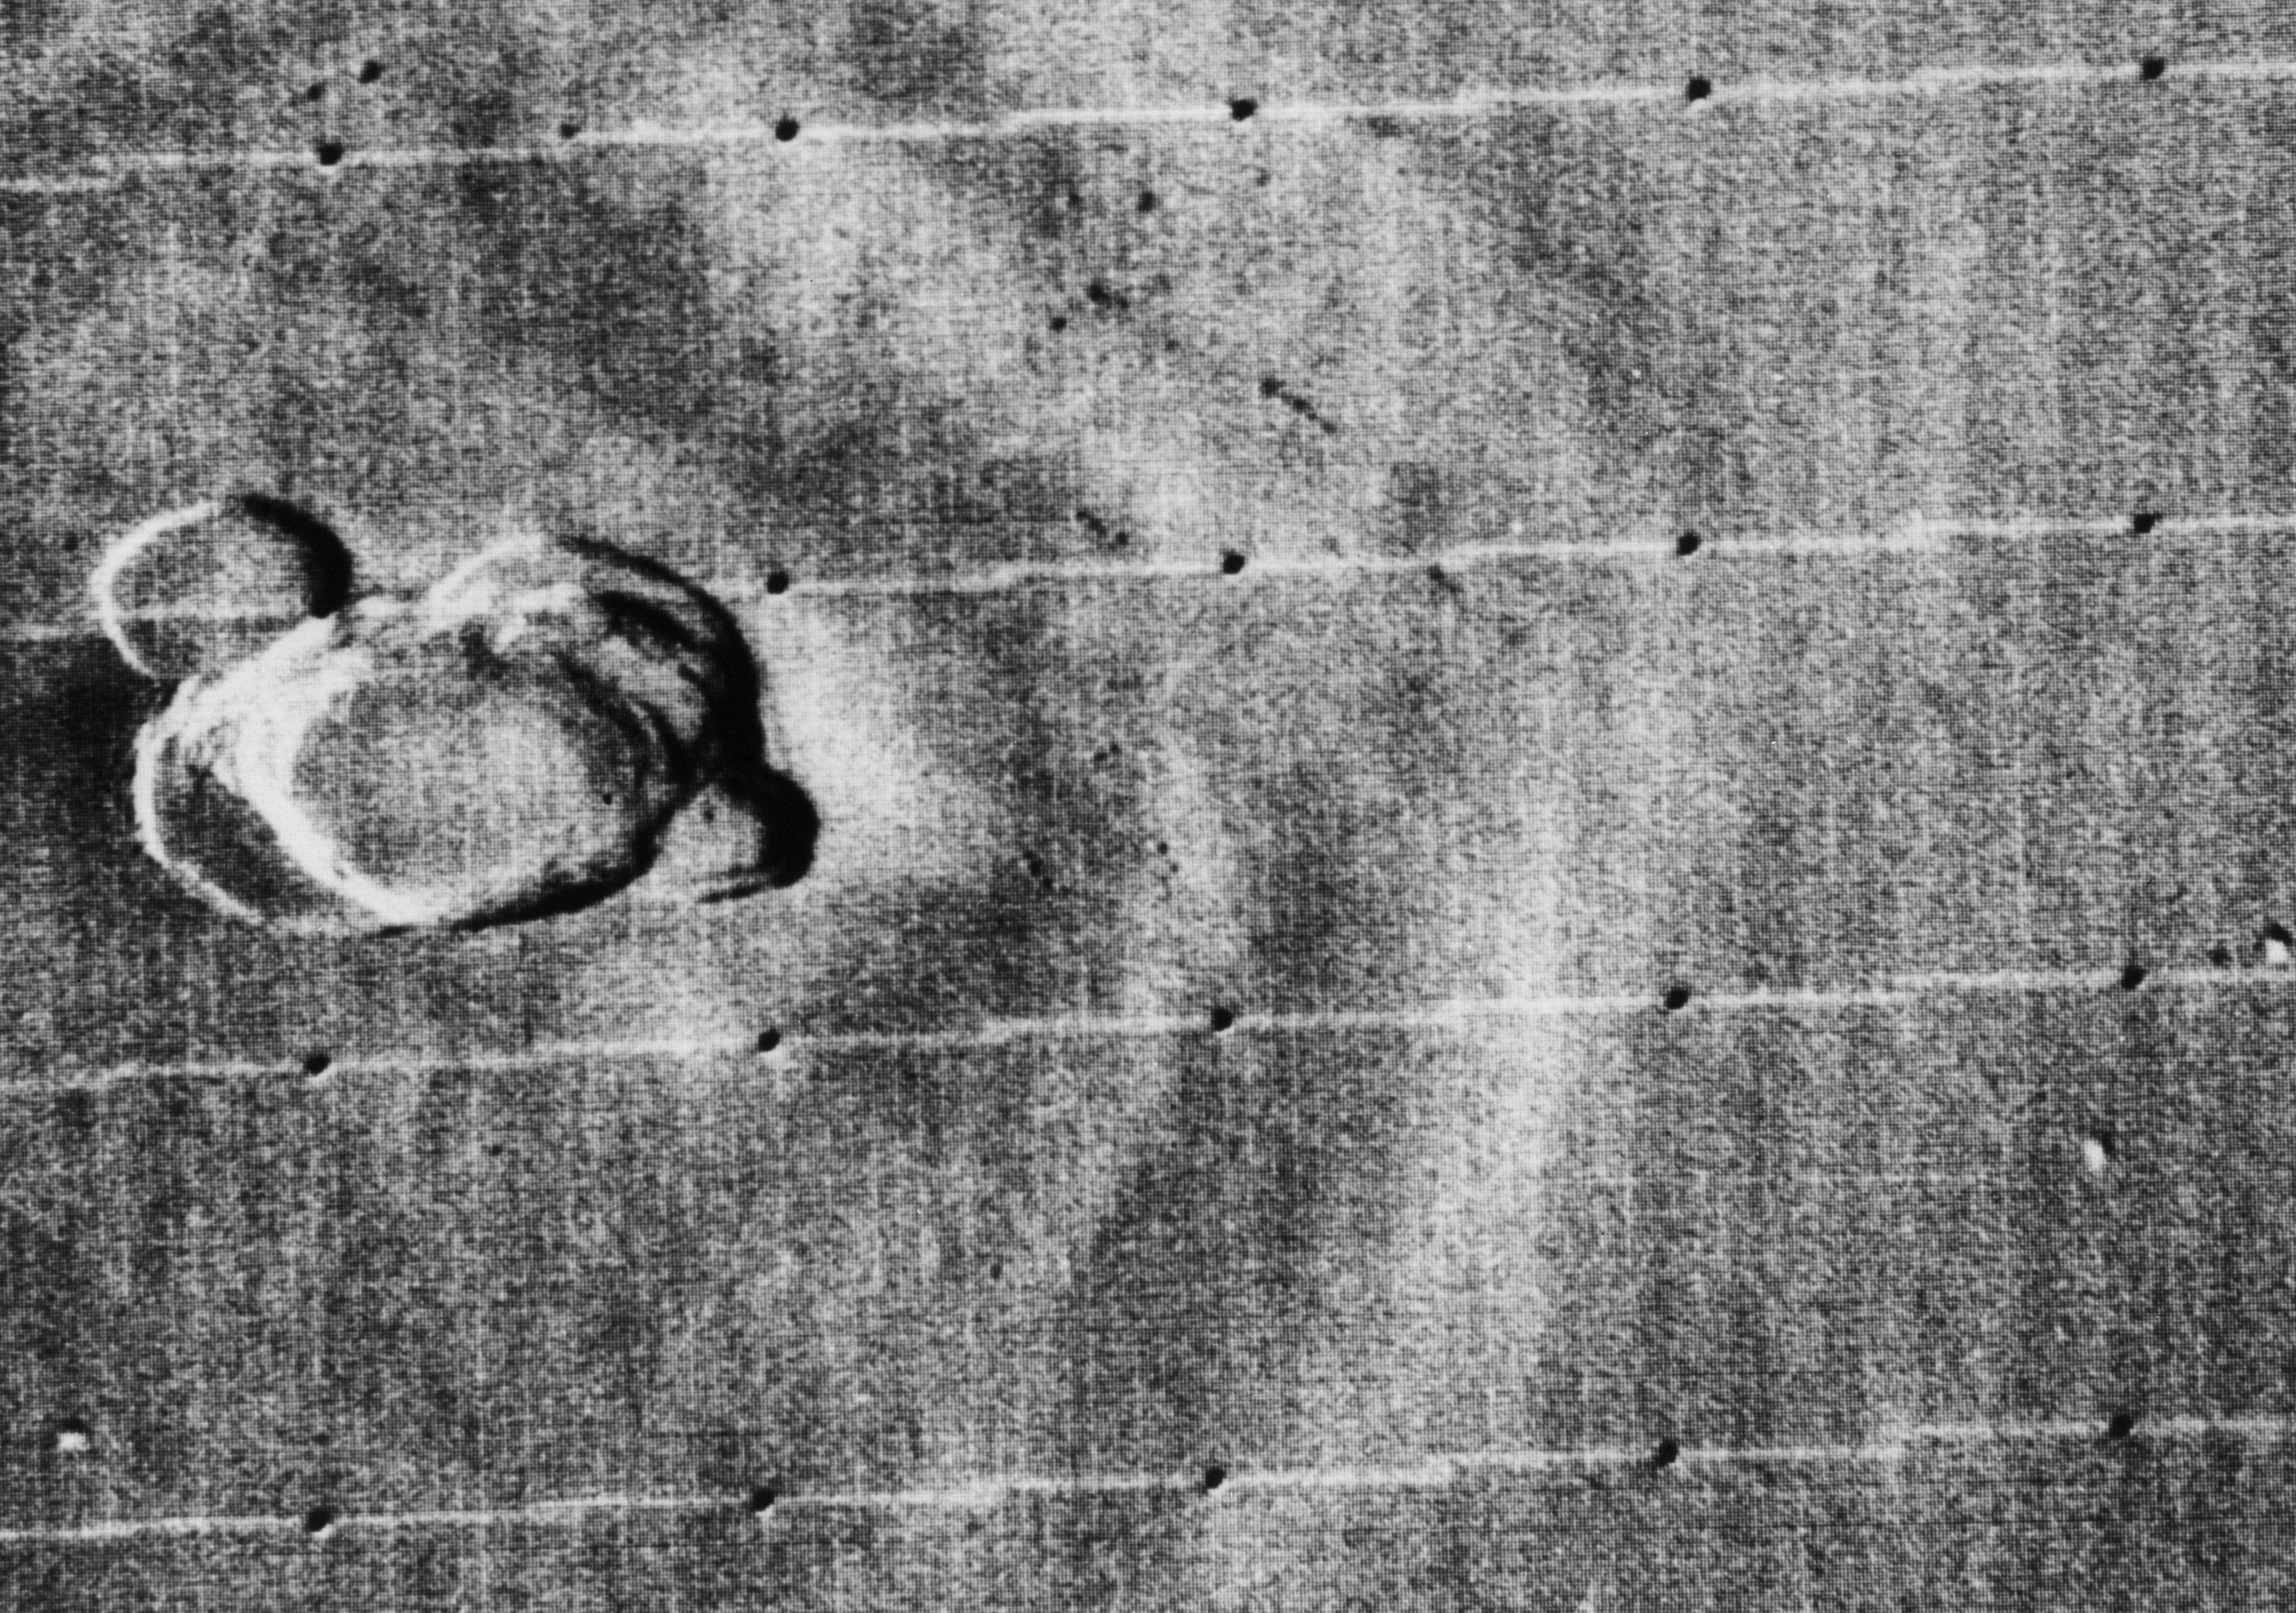
\includegraphics[scale=0.10]{mariner9.jpg}
\end{figure}
\end{frame}

%%%%%%%%%%%%%%%%%%%%%%%%%%%%%%%%%%%%%%%%%%%%%%%%%%%%%%%%


\begin{frame}
\frametitle{Construction}
$\V{x} \equiv (x_1,x_2,\ldots,x_m) \in \F^m$ 

$f(\V{x})$  \quad $f: \F_{2}^{m} \rightarrow \{0,1\} $ 
\newline

\begin {center}{Truth-Table}
\begin{tabular}{|c|c|c|c|c|c|c|c|c|}
\hline
$x_1$ & $0$ & $0$ & $0$ & $0$ & $1$ & $1$ & $1$ & $1$ \\
$x_2$ & $0$ & $0$ & $1$ & $1$ & $0$ & $0$ & $1$ & $1$ \\
$x_3$ & $0$ & $1$ & $0$ & $1$ & $0$ & $1$ & $0$ & $1$ \\
\hline
$f$   & $0$ & $1$ & $0$ & $1$ & $0$ & $1$ & $1$ & $0$ \\
\hline
\end{tabular}
\end{center} 
$\V{f}$ is a $n=2^m$ length vector over $F_2$

Disjunctive Normal Form : $f = x_3 + x_1x_2$  ( $+$ is \emph{xor} ) \\

A collection of $2^{2^m}$ vectors, each of length $2^m$.
\end{frame}

%%%%%%%%%%%%%%%%%%%%%%%%%%%%%%%%%%%%%%%%%%%%%%%%%%%%%%%%


\begin{frame}
 \frametitle{Boolean Monomials}
\begin{eqnarray*}
M &=& \{1,x_1,x_2,\ldots,x_m, x_1x_2,\ldots,x_{m-1}x_m,x_1x_2x_3,\ldots,x_1x_2\ldots x_m\}
\end{eqnarray*}
%%make the previous thing multi-line and nice looking.

\begin{equation*}
  f = 1 + a_1x_1+a_2x_2+\ldots+a_mx_m + a_{12}x_1x_2+\ldots+a_{12\ldots r}x_1x_2\ldots x_r+\ldots
\end{equation*}

Since $\V{f}$ is a linear combination, it follows that the length of $x_1, x_2,\ldots,x_m$ is $2^m$.
\end{frame}

%%%%%%%%%%%%%%%%%%%%%%%%%%%%%%%%%%%%%%%%%%%%%%%%%%%%%%%%


\begin{frame}
 \frametitle{Reed-Muller Codes}

\begin{block}{Reed-Muller codes}
The \alert{\rem{} codes} of order $r$ and length $n = 2^m$ ,$0 \leq r \leq m$  is the set of all vectors $\V{f}$, where $f(x_1,\ldots,x_m)$ is a Boolean function which is a polynomial of degree at most $r$.
\end{block}

\begin{block}{First-order codes}
 $\V{1}+a_1x_1+a_2x_2+\ldots+a_mx_m$
\end{block}
\end{frame}

%%%%%%%%%%%%%%%%%%%%%%%%%%%%%%%%%%%%%%%%%%%%%%%%%%%%%%%%

\begin{frame}
 \frametitle{Linearity}
\begin{Lemma}
  $\RM{r}{m}$ is a linear code.
\end{Lemma}

\begin{block}{Basis}
  The monomials of degree $\leq r$ form a basis for $\RM{r}{m}$.
\end{block}

Generator matrix
\begin{equation}
  \label{eq:5}
  G(r,m) =
  \begin{pmatrix}
    \V{1} \\
    \V{x_1} \\
    \V{x_2} \\
    \vdots \\
    \V{x_m} \\
    \V{x_1x_2} \\
    \vdots \\
    \V{x_1x_2\ldots x_r}
  \end{pmatrix}
\end{equation}

\end{frame}

%%%%%%%%%%%%%%%%%%%%%%%%%%%%%%%%%%%%%%%%%%%%%%%%%%%%%%%%

\begin{frame}
 \begin{block}{Dimension}
  The dimension ($k$) of $\RM{r}{m}$ is equal to the  number of monomials of degree $\leq r$ \quad $ k= 1+\binom{m}{1}+\binom{m}{2}+\ldots+\binom{m}{r} $
\end{block}

$\RM{0}{m} $ is the repetition code ($2^m$ repetition).\\
$\RM{m}{m}$ consists of all possible binary sequences of length $2^m$.

\begin{center}
\begin{tabular}[center]{|c|c|}
\hline
Length & $n = 2^m$ \\
Minimum Distance & $d = 2^{m-r}$ \\
Dimension & $k= 1+\binom{m}{1}+\binom{m}{2}+\ldots+\binom{m}{r}$ \\
\hline
\end{tabular}
\end{center}

\end{frame}

%%%%%%%%%%%%%%%%%%%%%%%%%%%%%%%%%%%%%%%%%%%%%%%%%%%%%%%%%%%%%

\begin{frame}
 \begin{equation*}

\RM{1}{3} = \begin{array}{|l|cccccccc|}
\hline
1 \quad&  	 1&1&1&1&1&1&1&1 \\
x_1 \quad& 	 0&0&0&0&1&1&1&1 \\
x_2 \quad& 	 0&0&1&1&0&0&1&1 \\
x_3 \quad&	 0&1&0&1&0&1&0&1 \\
x_1+x_2 \quad&    0&0&1&1&1&1&0&0 \\
x_1+x_3 \quad&	 0&1&1&0&0&1&1&0 \\
x_2+x_3 \quad&	 0&1&0&1&1&0&1&0 \\
x_1+x_2+x_3 \quad& 0&1&1&0&1&0&0&1 \\
1+x_1	\quad&	 1&1&1&1&0&0&0&0 \\
1+x_2	\quad&	 1&1&0&0&1&1&0&0 \\
1+x_3	\quad&	 1&0&1&0&1&0&1&0 \\
1+x_1+x_2 \quad&	 1&1&0&0&0&0&1&1 \\
1+x_1+x_3 \quad&	 1&0&0&1&1&0&0&1 \\
1+x_2+x_3 \quad&	 1&0&1&0&0&1&0&1 \\
1+x_1+x_2+x_3\quad& 1&0&0&1&0&1&1&0 \\
\hline
\end{array}
\end{equation*}
\end{frame}

%%%%%%%%%%%%%%%%%%%%%%%%%%%%%%%%%%%%%%%%%%%%%%%%%%%%%%%%%%%%%%

\begin{frame}
 \begin{equation*}
G(2,3) =\begin{array}{|l|cccccccc|}
\hline
1 \quad&         1&1&1&1&1&1&1&1 \\
x_1 \quad&       0&0&0&0&1&1&1&1 \\
x_2 \quad&       0&0&1&1&0&0&1&1 \\
x_3 \quad&       0&1&0&1&0&1&0&1 \\
x_1\cdot x_2 \quad& 0&0&0&0&0&0&1&1 \\ 
x_1\cdot x_3 \quad& 0&0&0&0&0&1&0&1 \\
x_2\cdot x_3 \quad& 0&0&0&1&0&0&0&1 \\
\hline
\end{array}
\end{equation*}
\end{frame}

%%%%%%%%%%%%%%%%%%%%%%%%%%%%%%%%%%%%%%%%%%%%%%%%%%%%%%%%%%%%%%

\begin{frame}
 \frametitle{Recursive Definition}
\begin{theorem}
\begin{equation*} \RM{r+1}{m+1} =  \{ \V{u} | \V{u}+\V{v} : \V{u} \in \RM{r+1}{m}, \V{v} \in \RM{r}{m} \} \end{equation*}
\end{theorem}

\begin{equation}
G(r+1,m+1) = \begin{pmatrix}
G(r+1,m) & G(r+1,m) \\
0 & G(r,m) 
\end{pmatrix}
\end{equation}

%We can also choose the vectors of the generator matrix in a systematic way 

\begin{equation}
G(1,m+1) = \begin{pmatrix}
G(1,m) & G(1,m) \\
0 & 1
\end{pmatrix}
\end{equation}
where
\begin{equation*}
  G(0,m) = ( {\overbrace{\V{1111}}^{2^m}} )
\end{equation*}

This way, the columns of $G(1,m)$ are binary representations of numbers from $1 \text{ to } 2^m$ in descending order.

\end{frame}

%%%%%%%%%%%%%%%%%%%%%%%%%%%%%%%%%%%%%%%%%%%%%%%%%%%%%%%%%%%%%%%%%%

\begin{frame}
 \begin{block}{Nested Structure}
\begin{equation*}
\RM{r}{m} \subseteq \RM{t}{m} \quad
\text{ if } 0 \leq r \leq t \leq m \\
\end{equation*}
\end{block}

\begin{theorem}
\label{general}
Let $C_i$ be an $[n,k_i,d_i]$ code. Then the concatenated code defined by

  \begin{equation*}
    C = \{(\V{u},\V{u}+\V{v}) | \V{u} \in C_1 , \V{v} \in C_2 \}
  \end{equation*}

has the parameters $[2n,k_1+k_2, min\{2d_1,d_2\}]$ .
\end{theorem}

\end{frame}

%%%%%%%%%%%%%%%%%%%%%%%%%%%%%%%%%%%%%%%%%%%%%%%%%%%%%%%%%%%%%%%%

\begin{frame}
 \frametitle{Properties}
\begin{block}{Distance}
Minimum distance, $d=2^{m-r}$
\end{block}

\begin{block}{First-Order}
\label{equidistant}
Every codeword in $\RM{1}{m}$ (except $\V{1}, \V{0}$) has weight $2^{m-1}$
\end{block}

\begin{block}{Dimension}
  \label{eq:1}
  \begin{equation*}
      dim(\RM{r}{m}) = dim(\RM{r}{m-1}) + dim(\RM{r-1}{m-1})
  \end{equation*}
\end{block}

\end{frame}

%%%%%%%%%%%%%%%%%%%%%%%%%%%%%%%%%%%%%%%%%%%%%%%%%%%%%%%%%%%%%%%%

\begin{frame}
\frametitle{Dual and Orthogonal of RM codes}
\begin{block}{Dual}
  $ \RM{m-r-1}{m} = \RM{r}{m}^{\bot} $
\end{block}

The dual code $\RM{1}{m}^{\bot}$ is the extended binary Hamming code $H(m)$ 

The \emph{Orthogonal code} $\mathcal{O}_m$ is a $[2^m, m, 2^{m?1}]$ code consisting of the vectors $ \sum_{i=1}^m{u_i\V{v_i}} $

\begin{block}{Orthogonal Code}
  $\RM{1}{m} = \mathcal{O}_m \cup (\V{1} + \mathcal{O}_m)$
\end{block}

\end{frame}

%%%%%%%%%%%%%%%%%%%%%%%%%%%%%%%%%%%%%%%%%%%%%%%%%%%%%%%%%%%%%%


\begin{frame}
 \frametitle{uniqueness}
\begin{theorem}
   Any linear code with parameters $[2^m, m+1, 2^{m-1}]$ is equivalent to the first order \rem{} code.
\begin{proof}
[Proof in \cite{uniq}]
\end{proof} \label{uniqness}
\end{theorem}
\end{frame}


%%%%%%%%%%%%%%%%%%%%%%%%%%%%%%%%%%%%%%%%%%%%%%%%%%%%%%%%%%%%%%

\begin{frame}
 \frametitle{Plotkin Bound}

\begin{theorem}[Plotkin Bound]
    If $C = [n,k,d]$ code, \begin{equation*}
d \leq \frac{n2^{k-1}}{2^k - 1}
\end{equation*}
  \begin{proof}
Counting in two ways:
\end{proof}
\end{theorem}


\end{frame}

%%%%%%%%%%%%%%%%%%%%%%%%%%%%%%%%%%%%%%%%%%%%%%%%%%%%%%%%%%%%%%%%%%%%%%%%%%%%%%%%

\begin{frame}
  \frametitle{Step Decoding}
\begin{Theorem}
One-step majority logic decoding can correct upto $\frac{n-1}{2(d'-1)}$ errors.\\
($d'$ is the minimum distance of the dual code.)
\begin{proof} 
$1 \quad \overbrace{1 1 1}^{\geq d'-1}  0 0 0 0 0 $ \\
$1 \quad 0 0 0  \underbrace{1 1 1 1 1}_{\geq d'-1} $

% Since there are $J$ such vectors.
% \begin{equation*}
%   J \leq \frac{n-1}{d'-1} 
% \end{equation*}
% \label{1stepdecode}
\end{proof}
\end{Theorem}  

\begin{block}{L-Step Decoding}
$E_L \leq \frac{n}{d'} - \frac{1}{2} $ 
% \begin{proof}
% Let the $i-th$ parity check involve $a_i$ coordinates (besides the $L$). 
% Since these checks correspond to the codewords in the dual code, we have

% \begin{eqnarray*}
% L+a_i &\geq& d' \\
% a_i + a_j &\geq& d'
% \end{eqnarray*}

% We also have 
% \begin{equation*}

% S = \sum_{i=1}^{J}{a_i} \leq n-L
% \end{equation*}
% Thus, \begin{eqnarray*}
% JL + S &\geq& Jd' \\
% (J-1)S &\geq& \binom{J}{2}d'
% \end{eqnarray*}
% Eliminating L and S: \begin{equation*}
% J \leq \frac{2n}{d' -1}
% \end{equation*}

%\end{proof}
\end{block}

L-step decoding can correct only 2 errors in Golay codes.

\end{frame}

%%%%%%%%%%%%%%%%%%%%%%%%%%%%%%%%%%%%%%%%%%%%%%%%%%%%%%%%%%%%%%%%%%%%%%%%%%%%%%%%

\begin{frame}
  \frametitle{Geometry}
  
\end{frame}

%%%%%%%%%%%%%%%%%%%%%%%%%%%%%%%%%%%%%%%%%%%%%%%%%%%%%%%%%%%%%%%%%%%%%%%%%%%%%%%%

\begin{frame}
  \frametitle{Reed Decoding Algorithm}
  \begin{block}{Algorithm}
    \begin{enumerate}
    \item For each row, find the $2^{m-r}$ \alert{characteristic vectors}, and take the dot product with $\V{x}$.
    \item The majority of the values of the dot products is the coefficient of the row (0/1) .
      \item Coefficient vector is the original message.
    \end{enumerate}
  \end{block}

  \begin{example}
Let $\V{m} = 0110$ in $\RM{1}{3}$. $\V{c} = 00111100$. $\V{x} = 10111100$.
  \end{example}
\end{frame}

%%%%%%%%%%%%%%%%%%%%%%%%%%%%%%%%%%%%%%%%%%%%%%%%%%%%%%%%%%%%%%%%%%%%%%%%%%%%%%%%

\begin{frame}
  \frametitle{Hadamard Transform}
\begin{def}
  The \emph{Real Vector} ${F(\V{v})}$ of a binary vector $\V{v}$ is a vector with $0$ replaced by $1$ and $1$ by $-1$.
\end{def}

  \begin{lem}
  The Orthogonal code $\mathcal{O}_m$ with real vectors is equivalent to the Hadamard matrix $H_m$.
\begin{proof}
    \begin{equation*}
      v_i, v_j \in \RM{1}{m} \implies v_i\cdot v_j = 0
    \end{equation*}
%    \begin{proof}
%      We can prove using induction on the basis vectors.\\
%Since the code is a linear combination, the result follows.
%    \end{proof}
$\mathcal{O}_m$ is a $2^m x 2^m$ matrix with elements $+1, -1$ such that dot product of any two rows is $0$.
\end{proof}
\end{lem}

\begin{equation}
  \label{eq:3}
  \RM{1}{m} =
  \begin{pmatrix}
    H_m \\
    -H_m
  \end{pmatrix}
\end{equation}

\end{frame}

\begin{frame}
  \frametitle{Fast Hadamard Transform}
Maximize the correlation between received vector $u$ and the rows:   \begin{equation*}
  corr(F(u),F(v)) = n - d(u,v)
\end{equation*}


\begin{thm}
  \begin{equation*}
    H_{2^m} = M_{2^m}^{(1)}M_{2^m}^{(2)} \ldots M_{2^m}^{(m)}
\text{\newline where \\}
  M_{2^m}^{(i)} = I_{2^{m-i}}\otimes H_2 \otimes I_{2^{i-1}}, \qquad 1 \leq i \leq m
  \end{equation*}
%  \begin{proof}
%    By simple induction on m.
%  \end{proof}
\end{thm}

Easy to implement in hardware --- used in Mariner-9. (Green Machine)
\end{frame}

%%%%%%%%%%%%%%%%%%%%%%%%%%%%%%%%%%%%%%%%%%%%%%%%%%%%%%%%%%%%%%%%%%%%%%%%%%%%%%%%

\begin{frame}
  \frametitle{List Decoding Algorithm}
Algorithm for $\RM{1}{m}$ capable of correcting $n(\frac{1}{2} - \epsilon)$ errors in $O(n \epsilon^3)$. \\
Hadamard Transform: $\frac{n}{4}$ errors in $O(n\log{n})$ time. \\


\begin{block} {Algorithm}
List: $L_{\epsilon}(y) = \{f \in \RM{1}{m} : d(\V{y}, \V{f} ) \leq n(\frac{1}{2} - \epsilon) \} $ \\
Candidate (ith prefix): $c^{(i)} (x_1 ,\ldots, x_m) = c_1x_1 + \ldots + c_ix_i$ \\
$ L_{\epsilon}^{(i)} (y) = \{c^{(i)}(x_1,x_2,\ldots,x_i) = c^{(i-1)}+c_ix_i\}$ \\
\begin{block}{distance}
  \Delta(\V{y},\V{c^{(i)}}) = \sum_\alpha|\V{y_\alpha}\V{c^{(i)}}| = \sum_\alpha|\V{v_\alpha^{(i)}}|
\end{block}
 \begin{equation*}
   S_{0,\alpha} =  \{(x_1,\ldots x_{i-1},0, \alpha_{i+1}\ldots \alpha_{m} \} 

 S_{1,\alpha} =  \{(x_1,\ldots x_{i-1},1, \alpha_{i+1}\ldots \alpha_{m} \} 
 \end{equation*}

Since $c^{(i)} = c^{(i-1)}+ c_ix_i$, we can write :
\begin{equation*}
  \V{v_\alpha^{(i)}} = \V{v_{0,\alpha}^{(i)}} + (-1)^{c_i}\V{v_{1,\alpha}^{(i-1)}}
\end{equation*}

\end{block}

\end{frame}

%%%%%%%%%%%%%%%%%%%%%%%%%%%%%%%%%%%%%%%%%%%%%%%%%%%%%%%%%%%%%%%%%%%%%%%%%%%%%%%%

\begin{frame}
  \frametitle{List Decoding}
  \begin{block}{Example}

\end{block}
\end{frame}

%%%%%%%%%%%%%%%%%%%%%%%%%%%%%%%%%%%%%%%%%%%%%%%%%%%%%%%%%%%%%%%%%%%%%%%%%%%%%%%%

\begin{frame}
  \frametitle{Applications}
  \begin{description}

\item[Communication]
Used in Mariner and Viking space-probes in the 1970's.
More recently, used is in the IEEE 802.11b standard for Wireless Local Area Networks (WLANs).

\item[Testing Low-degree polynomials]
Using $\RM{1}{m}$ codes to test whether a binary function is a low-degree polynomial is a central theme in a lot of research in complexity theory ~\cite{lowdeg} , ~\cite{local+testing}.In a typical scenario, the Boolean functions are mapped to the \rem{} codes, and the properties are used to prove the bounds on the number of queries needed to determine the original function.

\item[Sidelnikov cryptanalysis]
%The Sidenikov public-key system, (a variant of the McEliece cryptosystem) uses \rem{} codes instead of Goppa codes because of the efficient decoding ~\cite{sidelnikov}.
The cryptanalysis attack uses the properties of \rem{} codes to break the cryptographic code ~\cite{attack}. The uniqueness result stated earlier is a central feature in the cryptographic attack.~\cite{correlation}

\item[Side Channel attacks]
The list decoding of the $\RM{1}{m}$ codes is used in the side-channel attack described in ~\cite{roche}.

  \end{desription}
\end{frame}


\begin{frame}
  \frametitle{References}
  
\end{frame}

%%%%%%%%%%%%%%%%%%%%%%%%%%%%%%%%%%%%%%%%%%%%%%%%%%%%%%%%%%%%%%


\end{document}

\message{ !name(1.tex) !offset(-557) }
